
\documentclass[11pt, a4paper]{book}
\usepackage{svn-multi}
\svnid{$Id$}
\usepackage{prelim2e}
\renewcommand{\PrelimWords}{Draft Copy \svnkw{Id}}
%%\newcommand*{\mysvnrev}{\svnrev}
\usepackage[hyperindex=true,
			bookmarks=true,
            pdftitle={}, pdfauthor={Xi Yang},
            colorlinks=false,
            pdfborder=0,
            pagebackref=false,
            citecolor=blue,
            plainpages=false,
            pdfpagelabels,
            pagebackref=true,
            hyperfootnotes=false]{hyperref}
\usepackage[all]{hypcap}
\usepackage[palatino]{anuthesis}
\usepackage{afterpage}
\usepackage{graphicx}
\usepackage{amsmath}
\usepackage[ruled,vlined]{algorithm2e}

\usepackage{thesis}
\usepackage[square]{natbib}
\usepackage[normalem]{ulem}
\usepackage[table]{xcolor}
\usepackage{makeidx}
\usepackage{cleveref}
\usepackage[centerlast]{caption2}
\usepackage{float}
\urlstyle{sf}
\renewcommand{\sfdefault}{uop}
\usepackage[T1]{fontenc}
\usepackage[scaled]{beramono}
\usepackage{mwe}
\usepackage{multirow}


\renewcommand*{\backref}[1]{}
\renewcommand*{\backrefalt}[4]{
  \ifcase #1 %
    %
  \or
    (cited on page #2)%
  \else
    (cited on pages #2)%
  \fi
}




%      $Id: macros.tex 506 2009-10-05 16:57:07Z daniel $    

\usepackage{booktabs}
\usepackage{relsize}
\usepackage{xspace}
\usepackage{subfigure}
\usepackage{listings}
\lstloadlanguages{java}
\DeclareGraphicsRule{*}{pdf}{*}{}
\newcommand{\otoprule}{\midrule[\heavyrulewidth]}
\newcommand{\pldi}{ACM Programming Language Design and Implementation (PLDI)}
\newcommand{\taco}{ACM Transactions on Architecture and Code Optimization (TACO)}
\newcommand{\lctes}{ACM Languages, Compiler, and Tool Support for Embedded Systems (LCTES)}
\newcommand{\popl}{ACM Principles of Programming Languages (POPL)}
\newcommand{\ecoop}{European Conference for Object-Oriented Programming (ECOOP)}
\newcommand{\asplos}{ACM Architectural Support for Programming Languages and Operating Systems (ASPLOS)}
\newcommand{\sigmetrics}{ACM Measurement and Modeling of Computer Systems (SIGMETRICS)}
\newcommand{\oopsla}{ACM Object-Oriented Programming, Systems, Languages, and Applications (OOPSLA)}
\newcommand{\ismm}{International Symposium on Memory Management (ISMM)}
\newcommand{\veee}{ACM/USENIX Virtual Execution Environments (VEE)}
\newcommand{\micro}{ACM/IEEE International Symposium on Microarchitecture}
\newcommand{\isca}{ACM/IEEE International Symposium on Computer Architecture (ISCA)}
\newcommand{\icse}{International Conference  on Software Engineering (ICSE)}
\newcommand{\pact}{Parallel Architectures and Compilation Techniques (PACT)}
\newcommand{\casess}{ACM Compilers, Architectures, and Synthesis for Embedded Systems (CASES)}

\definecolor{tableheadcolor}{rgb}{0.8,0.8,1.0}
%\definecolor{tablealtcolor}{rgb}{0.9,0.9,1.0}
\definecolor{tablealtcolor}{rgb}{0.9,0.9,0.95}


\definecolor{todocolor}{rgb}{0.8,0.8,1.0}
\definecolor{fixcolor}{rgb}{1,0.8,0.8}
\definecolor{commentcolor}{rgb}{0.8,1.0,0.8}


\newcommand{\listingfigure}[3]{
\begin{figure}[ht!]
  \begin{center}
    \begin{minipage}[t]{\textwidth-4cm}
      \lstinputlisting{#1}
    \end{minipage}
  \end{center}
  \caption{#3}#2
\end{figure}}

\newcommand{\includeabchart}[5]{
\begin{figure}[ht!]
\begin{center}
\newcommand{\atitle}{#4}
\newcommand{\btitle}{#5}
\input{charts/#1.tex}
\end{center}
\caption{#3}#2
\end{figure}}

\newcommand{\placeholderfigure}[2]{
\begin{figure}[ht!]
  \begin{center}
    \resizebox{\textwidth-2cm}{0.7\textwidth-1.4cm}{todo}
  \end{center}
  \caption{#2}#1
\end{figure}}

\newcommand{\singlegraphfigure}[3]{
\begin{figure}[ht!]
  \begin{center}
    \includegraphics[width=\textwidth-2cm]{#1}
  \end{center}
  \caption{#3}#2
\end{figure}}

\usepackage[color=todocolor, colorinlistoftodos]{todonotes}

%\newcommand{\notinpart}{%
% \def\toclevel@chapter{-1}\def\toclevel@section{0}\def\toclevel@subsection{1}} \newcommand{\inpart}{
% \def\toclevel@chapter{0}\def\toclevel@section{1}\def\toclevel@subsection{2}}


%
% Stuff for pretty printing the source code using listings.sty
%


%% set Java as the default language
\lstset{
  numbers=left,
  numberstyle=\tiny,
  stepnumber=1,
  numbersep=2em,
  language=java,                         % the language
  basicstyle=\footnotesize\ttfamily,     % the basic font family to use
  commentstyle=\itshape,                 % the font for comments
  stringstyle=\ttfamily,
%  morekeywords={@Intrinsic, @Unboxed, @RawStorage}
}
%\lstset{language=java}

\newcommand{\textjava}[1]{{\lstset{basicstyle=\ttfamily}\lstinline@#1@}}
\newcommand{\textjavafn}[1]{{\lstset{basicstyle=\footnotesize\ttfamily}\lstinline@#1@}}
%\usepackage{lstasm}
\usepackage{setspace}
\usepackage{ifthen}
%\usepackage{color}
%\usepackage{smallheadings}

\long\def\sfootnote[#1]#2{\begingroup%
\def\thefootnote{\fnsymbol{footnote}}\footnote[#1]{#2}\endgroup}
%
% code
%

\newcommand{\address}{\textjava{Address}\xspace}
\newcommand{\ubregion}{\textjava{unbump-region()}\xspace}
\newcommand{\word}{\textjava{Word}\xspace}
\newcommand{\freeme}{\textjava{free()}\xspace}
\newcommand{\freemeunbump}{\textjava{unbump()}\xspace}
\newcommand{\freemeunbumpregion}{\textjava{unbump-region()}\xspace}
\newcommand{\freemeunreserve}{\textjava{unreserve()}\xspace}

%
% abbreviations
%


\newcommand{\eg}{e.g., }
\newcommand{\ie}{i.e., }

\newcommand{\GenMS}{\emph{GenMS}\xspace}
\newcommand{\GenImmix}{\emph{GenIX}\xspace}
\newcommand{\mmtk}{MMTk\xspace}
\newcommand{\jikes}{Jikes RVM\xspace} 
\newcommand{\jikesrvm}{\jikes} 
\newcommand{\jala}{Jalape\~{n}o\xspace} 
\newcommand{\jalapeno}{Jalape\~{n}o\xspace} 

\newcommand{\dacapo}{\textsf{DaCapo}\xspace}
\newcommand{\specjvm}{\textsf{SPECjvm98}\xspace}
\newcommand{\cattrack}{\textsf{cattrack}\xspace}
\newcommand{\spec}{\textsf{SPEC}\xspace}

\newcommand{\nurserytype}[1]{{\fontfamily{cmss}\selectfont \textsl{#1}}}
\newcommand{\alloc}{\nurserytype{allocate}\xspace}
\newcommand{\collect}{\nurserytype{collect}\xspace}
\newcommand{\redirect}{\nurserytype{redirect}\xspace}

\newcommand{\bmtype}[1]{{\textsf{#1}}}

\newcommand{\jbb}{\bmtype{jbb2000}\xspace}
\newcommand{\psjbb}{\bmtype{pjbb2005}\xspace}
\newcommand{\pjbb}{\bmtype{pjbb2005}\xspace}
\newcommand{\specjbb}{\bmtype{SPECjbb2005}\xspace}
\newcommand{\jess}{\bmtype{jess}\xspace}
\newcommand{\raytrace}{\bmtype{raytrace}\xspace}
\newcommand{\db}{\bmtype{db}\xspace}
\newcommand{\javac}{\bmtype{javac}\xspace}
\newcommand{\jack}{\bmtype{jack}\xspace}
\newcommand{\compress}{\bmtype{compress}\xspace}
\newcommand{\mpegaudio}{\bmtype{mpegaudio}\xspace}
\newcommand{\mtrt}{\bmtype{mtrt}\xspace}
\newcommand{\antlr}{\bmtype{antlr}\xspace}
\newcommand{\bloat}{\bmtype{bloat}\xspace}
\newcommand{\chart}{\bmtype{chart}\xspace}
\newcommand{\eclipse}{\bmtype{eclipse}\xspace}
\newcommand{\fop}{\bmtype{fop}\xspace}
\newcommand{\hsqldb}{\bmtype{hsqldb}\xspace}
\newcommand{\jython}{\bmtype{jython}\xspace}
\newcommand{\luindex}{\bmtype{luindex}\xspace}
\newcommand{\lusearch}{\bmtype{lusearch}\xspace}
\newcommand{\Lusearch}{\bmtype{Lusearch}\xspace}
\newcommand{\pmd}{\bmtype{pmd}\xspace}
\newcommand{\ps}{\bmtype{ps}\xspace}
\newcommand{\SPECjbb}{\bmtype{SPECjbb}\xspace}
\newcommand{\xalan}{\bmtype{xalan}\xspace}
\newcommand{\sunflow}{\bmtype{sunflow}\xspace}
\newcommand{\Sunflow}{\bmtype{Sunflow}\xspace}
\newcommand{\avrora}{\bmtype{avrora}\xspace}
\newcommand{\core}{Core2 Quad\xspace}
\newcommand{\corelong}{Intel Core2 Quad Q6600\xspace}
\newcommand{\phenom}{Phenom II\xspace}
\newcommand{\phenomlong}{AMD Phenom II X6 1055T\xspace}
\newcommand{\sandy}{i7-2600\xspace}
\newcommand{\sandylong}{Intel Core i7-2600\xspace}



\newcommand{\ghostscript}{\bmtype{ghostscript}\xspace}

\newcommand{\doi}[1]{\href{http://dx.doi.org/#1}{\nolinkurl{doi:#1}}}
%
% misc
%
\newcommand{\fix}[1]{\todo[color=fixcolor]{#1}}
\newcommand{\comment}[1]{\todo[color=commentcolor]{#1}}
\newcommand{\ifix}[1]{\todo[inline,color=fixcolor]{#1}}
\newcommand{\icomment}[1]{\todo[inline,color=commentcolor]{#1}}
\newcommand{\itodo}[1]{\todo[inline]{#1}}
\newcommand{\ignore}[1]{}
\newcommand{\mccenter}[1]{\multicolumn{1}{c|}{#1}}

%
% figure spacing
%
%\clubpenalty 10000
%\widowpenalty 10000
%\def\topfraction{0.9}
%\def\bottomfraction{0.9}
%\def\textfraction{0.1}
%\renewcommand{\singlespacing}{\renewcommand{\baselinestretch}{1.00}\small\normalsize}
%\renewcommand{\doublespacing}{\renewcommand{\baselinestretch}{1.5}\small\normalsize}
%\newcommand{\tight}{\renewcommand{\baselinestretch}{1.28}\small\normalsize}
%\renewcommand{\subfigbottomskip}{0.25ex}
%\renewcommand{\subfigcapskip}{0ex}
%\renewcommand{\subfigcapskip}{-1ex}
%\newcommand{\subfigshrink}{-0.75ex}
%\newcommand{\subfigcapspace}{2ex}

%\newcommand{\subwidth}[0]{.32\textwidth}


%
% margins
%
%\topmargin -.5truein
%\textheight 9truein
%\oddsidemargin .25truein
%\evensidemargin .25truein
%\textwidth 6truein


%
% crossreferencing footnotes
%
%\newcommand{\fnref}[1]{~(\ref{#1})}
%\newcommand{\onecolparbox}{3.1in}


%\newcommand{\textjava}[1]{{\lstset{language=java,basicstyle=\footnotesize\ttfamily}\lstinline@#1@}}
%\newcommand{\textasm}[1]{{\lstset{language=asm,basicstyle=\footnotesize\ttfamily}\lstinline@#1@}}

%%
%% Change the sections etc.
%%
%\makeatletter
%\parskip=0pt
%\renewcommand\section{\@startsection{section}{1}{\z@}%
%                                   {-2.5ex}% beforeskip
%%                                   {1ex}% afterskip
%                                   {\large \bfseries \raggedright}}
% \renewcommand\subsection{\@startsection{subsection}{2}{\z@}%
%                                     {-2ex\@plus -1ex \@minus -.2ex}%
%                                      {.5ex \@plus .2ex}%
%                                      {\normalsize \bfseries \raggedright}}
% \renewcommand\subsubsection{\@startsection{subsubsection}{3}{\z@}%
%                                      {-2ex\@plus -1ex \@minus -.2ex}%
%                                      {1ex \@plus .2ex}%
%                                      {\normalfont\fontsize{11pt}{12pt}\selectfont\itshape}}
%\renewcommand{\thesubsubsection}{\thesubsection.\arabic{subsubsection}}

%\renewcommand\paragraph{\@startsection{paragraph}{4}{\z@}% 
%  {.5em}%
%  {-1em}%
%  {\normalfont\normalsize\bfseries\parskip=0pt}}
%\setlength\partopsep{0\p@}
%\setlength\parskip{0\p@ \@plus \p@}

%\makeatother
%\parindent=9pt





%%% Local Variables: 
%%% mode: latex
%%% TeX-master: "doa"
%%% End:
            
%%%%%%%%%%%%%%%%%%%%%%%%%%%%%%%%%%%%%%%%%%%%%%%%%%%%%%%%%%%%%%%%%%%%%%%
%% Preamble
\title{An end to end Machine Learning Model for Compositional Data}
\author{Sean Lamont}
\date{\today}

\renewcommand{\thepage}{\roman{page}}

\makeindex
\begin{document}
%\doparttoc
%%%%%%%%%%%%%%%%%%%%%%%%%%%%%%%%%%%%%%%%%%%%%%%%%%%%%%%%%%%%%%%%%%%%%%%
%% Title page
\pagestyle{empty}
\thispagestyle{empty}
%% anuthesis.sty Copyright (C) 1996, 1997 Steve Blackburn
%% Department of Computer Science, Australian National University
%%

\begin{titlepage}
  \enlargethispage{2cm}
  \begin{center}
    \makeatletter
    \Huge\textbf{\@title} \\[.4cm]
    \Huge\textbf{\thesisqualifier} \\[2.5cm]
    \huge\textbf{\@author} \\[9cm]
    \makeatother
%%   \LARGE A thesis submitted for the degree of \\
%%    Master of Philosophy at \\
%%    The Australian National University \\[2cm]
    \LARGE A thesis submitted for the degree of \\
    Bachelor of Advanced Computing (Research and Development) (Honours) \\
    The Australian National University \\[2cm]
    \thismonth
  \end{center}
\end{titlepage}


%%%%%%%%%%%%%%%%%%%%%%%%%%%%%%%%%%%%%%%%%%%%%%%%%%%%%%%%%%%%%%%%%%%%%%%
%% Here begin the preliminaries
\vspace*{14cm}
\begin{center}
  \makeatletter
  \copyright\ \@author{} 2011
  \makeatother
\end{center}
\noindent
\begin{center}
  \footnotesize{~} %\aboutthesis
\end{center}
\noindent

\newpage

\vspace*{7cm}
\begin{center}
  Except where otherwise indicated, this thesis is my own original
  work.
\end{center}

\vspace*{4cm}

\hspace{8cm}\makeatletter\@author\makeatother\par
\hspace{8cm}\today


%%%%%%%%%%%%%%%%%%%%%%%%%%%%%%%%%%%%%%%%%%%%%%%%%%%%%%%%%%%%%%%%%%%%%%%
%% Dedication
\cleardoublepage
\pagestyle{empty}
\vspace*{7cm}
\begin{center}
to my xxx, yyy (yyy is the people you want to dedicated this thesis to.)
\end{center}


%%%%%%%%%%%%%%%%%%%%%%%%%%%%%%%%%%%%%%%%%%%%%%%%%%%%%%%%%%%%%%%%%%%%%%%
%% Acknowledgements
\cleardoublepage
\pagestyle{empty}
\chapter*{Acknowledgments}
\addcontentsline{toc}{chapter}{Acknowledgments}
Who do you want to thank?


%%%%%%%%%%%%%%%%%%%%%%%%%%%%%%%%%%%%%%%%%%%%%%%%%%%%%%%%%%%%%%%%%%%%%%%
%% Abstract
\cleardoublepage
\pagestyle{headings}
\chapter*{Abstract}
\addcontentsline{toc}{chapter}{Abstract}
\vspace{-1em}
  Compositional Data Analysis (CoDA) is the study of data which can be interpreted as ratios or counts. Data of this type manifests in many forms, from microbiome species counts to chemical compositions to wealth distributions. Compositional data is known to exist in a simplex, and so many standard statistical analysis methods (which assume Euclidean geometry) are unsuitable. The goal of this thesis is to expand on current dimensionality reduction research, and investigate the use of jointly optimising supervised learning  loss with the addition of a reconstruction error term. 
  
  There has been some progress in the analysis of this data, most of which centres on a log transformation which embeds the simplex in Euclidean space.  

%%% Local Variables: 
%%% mode: latex
%%% TeX-master: "paper"
%%% End: 

%%%%%%%%%%%%%%%%%%%%%%%%%%%%%%%%%%%%%%%%%%%%%%%%%%%%%%%%%%%%%%%%%%%%%%%
%% Table of contents
\cleardoublepage
\pagestyle{headings}
\markboth{Contents}{Contents}
\tableofcontents
\listoffigures
\listoftables

%%%%%%%%%%%%%%%%%%%%%%%%%%%%%%%%%%%%%%%%%%%%%%%%%%%%%%%%%%%%%%%%%%%%%%
%% Here begins the main text
\mainmatter

%% Introduction
\chapter{Introduction}
\label{cha:intro}


\section{Thesis Statement}
\label{sec:thesisstatement}
I believe A is better than B.


\section{Introduction}
\label{sec:problemstatement}
Put your introduction here. You could use \textbackslash fix\{ABCDEFG.\} to
leave your comments, see the box at the left side. \fix{You have to rewrite your
thesis!!!} 



\section{Thesis Outline}
\label{sec:outline}
How many chapters you have? You may have Chapter~\ref{cha:background},
Chapter~\ref{cha:design}, Chapter~\ref{cha:methodology},
Chapter~\ref{cha:result}, and Chapter~\ref{cha:conc}.


\section{Datasets}

3 good example microbiome datasets here:

https://microbiome.github.io/microbiome/Data.html

Using above package and phyloseq R package to process. 

\section{Notes}

Good Aitchinson ref:

%http://www.leg.ufpr.br/lib/exe/fetch.php/pessoais:abtmartins:a_concise_guide_to_compositional_data_analysis.pdf

In addition to techniques and mathematical analysis of the simplex, he also explains:

Hypersphere transformation to directional data is not reasonable (sphere and triangle are topologically different), and further criticises Dirichlet models 

Has more small (toy) datasets, and analyses which may be interesting to compare to. 


%% Chapters
\chapter{Background and Related Work}
\label{cha:background}
In this chapter we introduce the background and motivation for this project, and related work in the area. A summary of each section is given below.

\begin{itemize}
    \item Section \ref{sec:motivation}: This section details the main motivation for the project, including potential areas of application.
    \item Section \ref{sec:comp}: Here we introduce Compositional Data, outlining examples and areas of application. We then present the current methods used in the analysis of this data. 
    \item Section \ref{sec:dimred}: This section presents the topic of dimensionality reduction. We introduce the most common algorithm, PCA, as well as methods specific to compositional data. We also present several examples to illustrate the advantages of the different approaches.  
    \item Section \ref{sec:sup}: The main applications of supervised learning, regression and classification, are introduced here. 
\end{itemize} \pagebreak


\section{Motivation}
\label{sec:motivation}
There is an abundance of scientific data which can be considered compositional, which is to say that the components are non-negative and sum to a constant value. Any data which involves percentages or counts summing to a constant falls in this category, and so the scope of such data is very large. \\

Compositional data does not satisfy the standard assumptions which underlies many common methods of analysis. Despite this, it remains common practice to apply these methods to compositional data. This is particularly true for many microbiome studies, (for which we outline the necessary background in section \ref{microbiome}). As explained by \cite{Gloor2017}, these studies often ignore the compositional structure inherent to the data. Given the recent technological advancements in gene sequencing and the explosion of such data, appropriate analysis is crucial. Even if this structure is acknowledged, current methods for Compositional Data Analysis are severely lacking.   \\

The importance of Compositional Data Analysis is not restricted to microbiome studies, although this is an important area of application. Economic data (e.g. GDP and wealth distribution), chemical compositions, and geology (soil or rock compositions) are just a few examples of data which are compositional. The motivation of this project is thus given by the limitations of current Compositional Data Analysis, and the large scope of applications where it is necessary.   



\section{Compositional Data}
\label{sec:comp}

\subsection{Definition}
As stated earlier, compositional data consists of a set of non-negative vectors which sum to a constant value (this is usually normalised to be 1 so the components can be interpreted as percentages of a whole). Formally, a compositional matrix $\mathbf{X} \in \mathbb{R}^{n\times d}$ will have each row vector $x_i \in \mathbb{R}^d$ as an element of the $d-1$ dimensional simplex, which is defined as: $$S^{d-1} = \{s \in \mathbb{R}^d : \sum_{i=1}^{d}s_i = c\}$$ for a fixed constant $c$ (that is, each column vector $x_i$ must sum to $c$). We note that the simplex is of dimension $d-1$ because we can determine the final component from the sum of the rest, given that $c$ is a fixed constant. More precisely, the final component of a compositional vector $x_i$ is clearly $(x_i)_{d} =  c - \sum_{j=1}^{d-1}(x_i)_j$ and so $x_i$ is of dimension $d-1$.   


\subsection{Example: RGB and the 2D simplex}
An example which illustrates this concept well is the RGB triangle. Any colour in RGB format can be interpreted as a composition of each of the colours Red, Green and Blue. In the notation above, this corresponds to a vector in $\mathbb{R}^3$.
Figure \ref{fig:rgbsimplex} gives a visual representation of the simplex of all such vectors. 

\usetikzlibrary{fadings}
\begin{figure}
 \begin{center}
\subfigure[An RGB Colour Triangle is an example of a 2D simplex in 3D space]{  
   
       \begin{tikzpicture}
      \fill[green] (90:4) -- (210:4) -- (-30:4) -- cycle;
      \fill[blue,path fading=west] (90:4) -- (210:4) -- (-30:4) -- cycle;
      \fill[red,path fading=south] (90:4) -- (210:4) -- (-30:4) -- cycle;
    \end{tikzpicture}
}

\subfigure[The standard 2D simplex as a subset of $\mathbb{R}^3$. The shaded region corresponds to the set $S^{2} = \{\mathbf{x} \in \mathbb{R}^3 : x_1 + x_2 + x_3 = 1\}$]{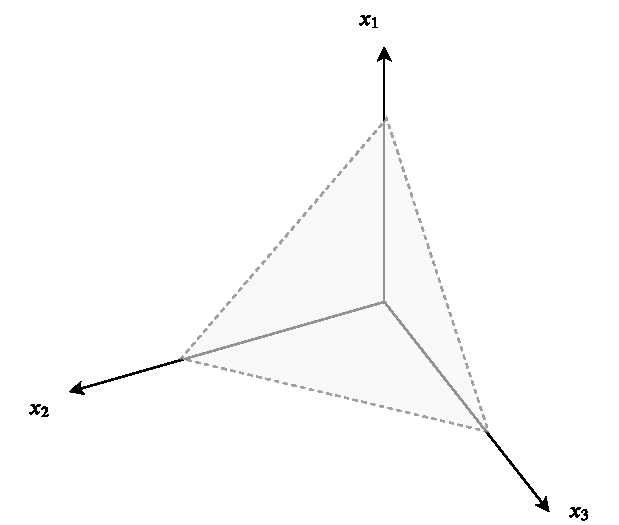
\includegraphics[]{figs/2dsimplex(2)(1).pdf}}

    \caption{The 2D Simplex}
    \label{fig:rgbsimplex}
    
\end{center}
\end{figure}




Using this example, we note several points: 
\begin{itemize}
    \item The total magnitude of the vector $(R,G,B)$ is irrelevant to the colour produced. What is important it the relative magnitudes between the values $R,G,B$. This is why we can normalise compositions to $1$ without losing or distorting information.   
    \item The simplex is fully defined as a 2D subset of $\mathbb{R}^3$, as it is a triangle. In general, the simplex extends the triangle to higher dimensions.  
    \item The maximum value any of $R,G,B$ can take is given by each of the vertices.
    \item A gain in any particular $R,G,B$ will correspond to that amount lost between the other values. This is the qualitative interpretation of the restriction that the parts must sum to a fixed value. 
\end{itemize}
\pagebreak



 
\subsection{Compositional Data Analysis (CoDA)}
\label{coda}
Given compositional data lies on the simplex, analysis of these data are complicated by the fact that they exist in a non-Euclidean mathematical space. As such, any attempt to compare distances between elements of this space cannot take place in the standard manner. The study of Compositional Data is known as Compositional Data Analysis (CoDA for short) and \cite{Aitchison1982} was the first to treat this issue in depth. At the core of Aitchinson's approach was the idea of a log transformation. For a point on the simplex, applying these transformation embeds the point in Euclidean space facilitating standard distance comparisons. There are several of these transformations, however these all lead to similar results as they only differ by a linear transformation. The most widely used (and most applicable for this project) is the centered log ratio (clr) transformation. Using notation from \cite{Avalos2018}, the clr transformation is formally defined as: $$\mathbf{c}_{KL}(\mathbf{x}) = \log \left(\frac{x}{(\prod_{j=1}^d x_j)^{\frac{1}{d}}}\right)$$  

We note that $\mathbf{c}_{KL} : S^{d-1} \to  \mathbb{R}^d$ is a bijective map from $S^{d-1}$ to  $\mathbb{R}^d$ by observing the inverse function which is given by 
$$\mathbf{c}_{KL}^{-1}(\mathbf{x}) = e^\mathbf{x} \prod_{i=1}^d e^{\frac{x_j}{1-d}}$$ ...

\section{Dimensionality Reduction}
\label{sec:dimred}

A concept crucial to this thesis is dimensionality reduction. Broadly, this refers to the set of techniques used to represent high dimensional data in a reduced form. Formally, we consider a data matrix $X \in \mathbb{R}^{d \times n}$ with $n$ elements, each with dimension $d$. The goal of dimensionality reduction is then to find what we denote as a representation matrix $A \in \mathbb{R}^{l \times n}$, where $l < d$. Since $l < d$, each column $x_i \in \mathbb{R}^d$ of $X$ will map to a lower dimensional representation $a_i \in \mathbb{R}^l$. This can be interpreted as projection of $x_i$ to a new coordinate system. In practice, it can be useful to consider $A$ as an encoding of $X$. We can then reconstruct an approximation to the original matrix $X$ through a decoding matrix $V \in \mathbb{R}^{l \times d}$. Through this we can obtain a reconstruction of $X$ of the same dimension, which is given by $V^TA \in \mathbb{R}^{d \times n}$. 

Motivation? (Smaller size, noise,  \citep{Shlens2005}: physics example, redundancy, signal to noise ratio)

There are many different approaches to dimensionality reduction, which seek to find $A$ based on different criteria and assumptions on the underlying data $X$. These approaches can be considered as minimising a distortion (generalised distance)  between functions of the reconstruction $V^TA$ and the orignal matrix $X$. This interpretation was particularly helpful for the paper which inspired this project \citep{Avalos2018}. Below we outline those dimensionality reduction techniques relevant to this research.    

\subsection{Principal Component Analysis (PCA)}
The most well known dimensionality reduction method is Principal Component Analysis (PCA) \citep{MackiewiczRatajczak1993}. There are several different interpretations of PCA, including SVD, covariance, etc... An intuitive explanation is given by \cite{Shlens2005}, which we draw from. PCA seeks to find a representation matrix $A$ where the covariance matrix of $A$ is diagonalised. As explained by \cite{Shlens2005}, this is desirable as each basis vector for the new coordinate system is uncorrelated, which minimises the shared information between them. This representation can be... 

\subsection{Exponential Family PCA}
Exponential family PCA: Extends PCA analogous to GLMs extending Linear Regression to exponential family. In the same way, allows for loss functions which are more appropriate for the parameter space, where parameters can be non Gaussian. Main example is count data i.e. Poisson which is exponential family. Situation is when data space (e.g. Poisson) is different to parameter space e.g. Reals

\subsection{CoDA-PCA}
\label{codapca}
This thesis primarily builds upon the 2018 NIPS paper on Representation Learning for Compositional Data \citep{Avalos2018}. The main result of the paper is the algorithm CoDA-PCA, which is a method for dimensionality reduction of compositional data. The standard approach to dimensionality reduction prior to this result was to apply PCA to the clr transformed data. CoDA-PCA combines clr with exponential family PCA, which allows PCA to be applied to count data. This simultaneously keeps the data centered through clr, and makes use of a loss function which considers the count nature of the data in the reconstruction error. The improvement can be seen dramatically in the ARMS example presented in the paper, where we see that CoDA-PCA and its variants are the only algorithms which faithfully represent the original data \citep{Avalos2018}, and our software can reproduce this result (Chapter \ref{cha:result}).     



 

(Maybe have chapter/section on the early experiments with CoDA-PCA, compared to CLR etc. on Aitchinson data)


\section{Supervised Learning}
\label{sec:sup}


\subsection{Regression}
\subsubsection{Definition}
One of the most widely used supervised learning methods is Linear Regression. The setup of regression is simply to estimate a target $y \in \mathbb{R}$ through a linear transformation of the features $\mathbf{x} \in \mathbb{R}^{d}$. For a single observation $\mathbf{x}$, this is done through the weight vector $\mathbf{w}$. The predicted value for $\mathbf{x}$ is then given by:
\begin{align}
    \hat{y} = \mathbf{w}^T\mathbf{x}
\end{align}

The goal is then to find $\mathbf{w}$ such that the predictions are as close as possible to the ground truth $y$. There is no single solution to this problem, as different formulations of distance give different results on how "close" the fit is. For example, one might prefer the properties of the $l_1$ distance $\sum_{i=1}^n|\hat{y}_i - y|$ over the $l_2$. The choice of distance in turn influences the optimal weights, since the weights are chosen to minimise this distance. In most practical applications, the model weights are chosen to optimise the $l_2$ loss, which we define as
\begin{align}
    l_{\mathrm{regression}} &= ||\mathbf{\hat{y}} - \mathbf{y}||_2^2 \\
    &= \sum_{i=1}^n  ||\hat{y} - y||_2^2 \\
     &= \sum_{i=1}^n  ||\mathbf{w}^T\mathbf{x} - y||_2^2 \\
    &= ||\mathbf{X}\mathbf{w} - \mathbf{y}||_2^2 
    \label{regressionloss}
\end{align}

This is often referred to as Ordinary Least Squares (OLS) regression, as it minimises the square $l_2$ loss. This is the loss function we assume for regression throughout the thesis.


\subsubsection{Optimal Parameters}
The optimal model parameters for the $l_2$ case can be found by minimising the loss in \ref{regressionloss} with respect to the weights: 
\begin{align}
    \mathbf{w}^* = \arg \min_{\mathbf{w}}l_{\mathrm{regression}} = \arg \min_{\mathbf{w}} ||\mathbf{X}\mathbf{w} - \mathbf{y}||_2^2 
\end{align}

This can easily be solved by matrix calculus:
 
 \begin{align*}
     ||\mathbf{X}\mathbf{w} - \mathbf{y}||_2^2  &= (\mathbf{X}\mathbf{w} - \mathbf{y})^T(\mathbf{X}\mathbf{w} - \mathbf{y}) \\
     &= \mathbf{w}^T\mathbf{X}^T \mathbf{X}\mathbf{w} - \mathbf{y}^T\mathbf{X}\mathbf{w} - \mathbf{X}^T\mathbf{w}^T\mathbf{y} - \mathbf{y}^T\mathbf{y}
 \end{align*}
 
 Since we are minimising with respect to $\mathbf{w}$, we can omit $\mathbf{y}^T\mathbf{y}$. Since all the terms are scalars, we may also note that $\mathbf{y}^T\mathbf{X}\mathbf{w} = (\mathbf{y}^T\mathbf{X}\mathbf{w})^T = 
 \mathbf{X}^T\mathbf{w}^T\mathbf{y} $. 
 
 Therefore: 
\begin{align*}
    \mathbf{w}^* &= \arg \min_{\mathbf{w}}l_{\mathrm{regression}} \\ 
    &= \arg \min_{\mathbf{w}} \mathbf{w}^T\mathbf{X}^T \mathbf{X}\mathbf{w}  - 2\mathbf{X}^T\mathbf{w}^T\mathbf{y} \\
    \nabla_{\mathbf{w}} l_{\mathrm{regression}} &= 2
\mathbf{X}^T \mathbf{X}\mathbf{w} - 2\mathbf{X}^T\mathbf{y}
\end{align*}
Setting this to $0$ gives us:
\begin{align*}
2
\mathbf{X}^T \mathbf{X}\mathbf{w} - 2\mathbf{X}^T\mathbf{y} &= 0 \\
\mathbf{X}^T \mathbf{X}\mathbf{w} &= \mathbf{X}^T\mathbf{y} \\
\mathbf{w} &= (\mathbf{X}^T \mathbf{X})^{-1}\mathbf{X}^T\mathbf{y}
\end{align*}

This solution is a minimum of the loss function $l_{\mathrm{regression}}$ since the Hessian $2\mathbf{X}^T\mathbf{X}$ is positive definite for all $\mathbf{X}$. Therefore the optimal set of weights for the $l_2$ regression loss is given by 
\begin{align}
    \mathbf{w}^* &= (\mathbf{X}^T \mathbf{X})^{-1}\mathbf{X}^T\mathbf{y}
\end{align}

\subsubsection{Regression Example: }
Here we present an example application of regression, 



\subsubsection{Principal Component Regression}
A common approach in regression problems is to apply dimensionality reduction on the features, and use the resulting representation as input for the regression. This is particularly useful for large feature spaces, and can improve model performance and efficiency. We expand on why this occurs in \ref{reconerror}. When PCA is used, this approach is known as Principal Component Regression (PCR). 


https://blogs.sas.com/content/iml/2017/10/25/principal-component-regression-drawbacks.html
PCR (PCA then Regression), does not consider the response in choosing the representation. No a priori reason to use the components of maximum variance.

\subsection{Classification}
\subsubsection{Definition}
The other key supervised learning problem is classification. In a classification task, the targets $\mathbf{y}$ are now in a discrete set $\{1, ..., k\}$ which we call the classes. Given an observation $\mathbf{x} \in \mathbb{R}^{d}$, the goal is then to predict which class it belongs to i.e. learn a mapping $\mathbf{x} \to \mathbf{y} \in \{1, ..., k\}$. This is referred to as a multi class classification problem, in contrast to the binary case where $\mathbf{y} \in \{0,1\}$. There are myriad ways to solve this problem in the literature. We focus on the multi class logistic regression approach, as the associated loss function will be needed for our model. 

\subsubsection{Multi class Logistic Regression}
Multi class Logistic Regression approaches the classification problem through combining a softmax function with a linear transformation of the features. Formally, for a vector $\mathbf{x}\in \mathbb{R}^d$ we define softmax as a function on each component $x_i \in \mathbf{x}$:

\begin{align}
   S(x_i) = \frac{e^{x_i}}{\sum_{x_i \in \mathbf{x}}e^{x_i}} 
\end{align}

As with Regression, we have a linear transformation of the features $\mathbf{w}^T\mathbf{x}$. The softmax is then applied to this transformation, which gives the predicted probabilities for each class: 

\begin{align}
   \mathbb{P}(\hat{y} = j | \mathbf{w}^T\mathbf{x}) &= S((\mathbf{w}^T\mathbf{x})_j)\\
   &=  \frac{e^{(\mathbf{w}^T\mathbf{x})_j}}{\sum_{i=1}^{k} e^{(\mathbf{w}^T\mathbf{x})_i}} 
\end{align}

The prediction is then taken as the maximum of these probabilities:

\begin{align}
   \hat{y} &= \arg \max_j S((\mathbf{w}^T\mathbf{x})_j)\\
   &= \arg\max_j \frac{e^{(\mathbf{w}^T\mathbf{x})_j}}{\sum_{i=1}^{k} e^{(\mathbf{w}^T\mathbf{x})_i}} 
\end{align}

\subsubsection{Negative Log Likelihood}
To learn the weights $\mathbf{w}$, we again must optimise a loss function. The loss function which we use is the Negative Log Likelihood. We justify the use of this loss function by considering the likelihood expression for $\mathbf{y}$.  

as being which is justified as it is minimising the negative (maximising the positive) of the log (monotone transformation) of the likelihood. 




\section{Microbiome}
\label{microbiome}
One of the main fields of interest for Compositional Data Analysis is microbiome studies. At a high level, a  microbiome refers to the community of simple organisms (e.g. bacteria) which occupy a particular location on any complex organism (e.g. humans). This is a rapidly growing subfield of genomics, as it can reveal relationships which exist between the microbiome and the external environment. One of the main applications of this includes studying the human microbiome to investigate its connection to health and disease, with the American Gut Project \citep{McDonalde00031-18} making recent progress in this area.

\subsection{Genomics and Gene Sequencing}
Before we can understand how CoDA is relevant for Microbiome studies, we must cover what exactly the data is and how it is collected. As mentioned above, microbiome data is collected to reveal information about the distribution of smaller organisms in a particular site on another larger organism (the human gut microbiome, for example). The goal is to fully describe this microbial community by the abundance of each organism inside it. Figure xx outlines the high level pipeline of the data retrieval and processing steps to obtain this abundance data. The first step is to sequence the community of interest. There are two broad approaches to this, which are discussed in \ref{16s} and \ref{metagenome}: Marker gene sequencing (usually 16S sequencing), and metagenomic 'shotgun' sequencing. Once this is completed, the next step is to use the resulting sequences to infer the frequencies of the organisms present in the microbiome. This is dependent on the sequencing method used, and in practice it is difficult to map from sequences to frequencies. One problem is how the sequences are mapped to individual organisms. This is again highly dependent on the sequencing method, which we detail in the following sections. 



\subsubsection{16S Sequencing}
\label{16s}
Although many species have been identified to date, there are a vast number of microorganisms which do not fit into the current taxonomy. This poses a large problem, as such organisms cannot be classified by reference to those that are currently known.One solution to the problem is to use Operational Taxonomic Units, or OTUs. This relates to one of the common gene sequencing methods, 16S. In this sequencing paradigm, only a single gene (the 'marker' gene) is sequenced for a given sample, which is usually the 16S rRNA gene. This specific gene is used since it is common to all bacteria, and its function has changed minimally over time. Variations in the 16S gene can therefore be linked to the evolution of an organism. For example, a similarity of below 97\% between 16S sequences is widely considered to distinguish organisms at the species level (https://jcm.asm.org/content/jcm/45/9/2761.full.pdf). These similarities are then used to construct OTUs, grouping organisms into a single OTU if they fall within a threshold value (e.g. 97\% for species). From this, an OTU table is constructed which contains counts of each OTU per sample. This data is intrinsically compositional, since the total read count of the instrument is fixed, and so the OTU counts are relative proportions \citep{Gloor2017}. These OTUs can be constructed without reference to an existing database, however...


\subsubsection{Metagenomic Sequencing}
\label{metagenome}




There has recently been significant progress in gene sequencing methods, resulting in an abundance of new microbiome data. These methods serve to provide an indication of the relative abundance of microbial species at a particular location (usually stomach or stool). (ref) It is known that microbiome data is inherently compositional, however this is often overlooked in its statistical analysis. In particular, standard PCA is often applied, which as we have seen can lead to poor representations and therefore misleading conclusions.  

Low dimensional representation of compositions good, since microbiomes can have very large feature space. Reduces space, time, avoids curse of dimensionality. 

- Metagenomics vs 16S: 16S analyses sequence a single gene across organisms, whereas metagenomic sequencing maps the genome of each organism. This allows for a more detailed representation of the underlying microbiome community. "meta" since it maps all genomes of different organisms. Assembly of genomes (the entire DNA content of an organism, needed for it to "build and maintain the organism") involves piecing together whole genome from sequences of reads of base pairs (using e.g. shotgun sequencing which gets a large collection of fragments, not necessarily linked). Metagenomics is therefore prone to errors, requiring the reads to be organised and mapped to genomes of particular organisms. E.g. Chimeric contigs (contiguous sequences of DNA mapped from different species).   

Useful for comparisons between organisms metagenomes, compare taxonomic content between organisms and assess for statistical difference (compositional!) https://www.ncbi.nlm.nih.gov/pmc/articles/PMC3044276/ 



\subsection{Reconstruction Error}
\label{reconerror}
 It is widely known that the use of dimensionality reduction prior to the application of supervised learning models can improve performance (see, for example, \cite{HOWLEY2006363}). There is some speculation as to exactly why this is the case, as these methods reduce the amount of information present in the data. The improvement in accuracy is mostly seen for high dimensional data, for which the widely known "curse of dimensionality" reduces model performance. The reduction of the input dimension facilitates lower computational cost and faster convergence of algorithms, and so greater performance. In practical cases of small training examples, higher dimensional data prevents many models from recognising patterns in noisy data. It is also claimed that principal components explaining less variance correspond to noise in the data. Under this view, the removal of these components would help to reduce overfitting by ensuring the model is fitted only to the useful parts of the data. Whatever the reason, supervised learning performance can be improved by dimensionality reduction on the features, and this forms the motivation for our model. Conventionally, dimensionality reduction is first performed to obtain a low level representation of $X$, which we denote as $A$. The matrix $A$ is then used as input to a supervised learning algorithm. Such an approach constructs $A$ with no regard to the performance of the supervised learning, only optimising based on a reconstruction loss. 




\section{Related work}
\label{sec:relatedwork}




\section{Summary}
Summary what you discussed in this chapter, and mention the story in next
chapter. Readers should roughly understand what your thesis takes about by only reading
words at the beginning and the end (Summary) of each chapter.




\chapter{Design and Implementation}
\label{design}
In this chapter we introduce a novel model for Compositional Data Analysis. It combines dimensionality reduction and supervised learning into a single, end-to-end algorithm. This design is motivated by the drawbacks of traditional methods, such as PCR. Such methods obtain the low level representation independently of the training targets, and so may ignore information which can improve the predictive performance. We divide this chapter into the following sections: 

\begin{itemize}
    \item Section \ref{design}: Here we present a high level overview of the model, including the assmuptions, inputs and outputs. 
    \item Section  \ref{endloss}: This section describes in detail the loss function(s) which the model is optimising.
    \item Section \ref{architecture}: The full architecture of the model is outlined here. We also detail the computations involved in a forward pass of the model. 
    \item Section \ref{implementation}: The implementation details of the model are presented and discussed here. We also detail the Python package for this code, which is available online.
\end{itemize}
\pagebreak



\section{Model Overview}
\label{design}
The application of our model is to supervised learning problems where the features form a compositional data set. The targets are currently restricted to single real valued numbers (regression), or classification problems (either single or multi class). Formally, the model takes as input a compositional matrix $\mathbf{X} \in \mathbb{R}^{n \times d}$ with each $x_i \in S^{d-1}$.  The output of the model is a prediction $\hat{\mathbf{y}}$ of the true targets $\mathbf{y}$. In the regression case, the targets are $\mathbf{y} \in \mathbb{R}$, and for classification $\mathbf{y} \in \{0, ..., k\}$ where $k$ is the number of classes. The prediction is generated from the following two steps:
\begin{itemize}
    \item Reduce $X$ to a representation $A \in \mathbb{R}^{n \times l}$ where $l < d$, through the mapping $\Theta(X) = A$.
    \item Use $A$ as input to the prediction mapping, which we denote as $r(A) = \mathbf{\hat{y}}$.
\end{itemize}

\todo{Introduce notation. How you stack elements into vectors, vectors into matrices, bold, non-bold, etc}

We can then define the end-to-end mapping from $X$ to $\mathbf{\hat{y}}$ as the composition of the above functions:
\begin{align}
\label{forwardpass}
    f(X) = r(\Theta(X)) = r(A) = \mathbf{\hat{y}}
\end{align}

\section{End to End Loss}
\label{endloss}
The steps outlined above for the forward pass are common to many supervised learning approaches, such as PCR which also performs regression on a low level representation. The novelty of our approach is the loss function under which $f(X)$ is optimised. In typical applications, the encoding $\Theta(X)$ and the prediction $r(A)$ are separately optimised with respect to different criteria. To account for this, our model instead directly optimises the composition $f(X)$ under a single loss function. \\
\fix{Careful of bold vs non-bold. E.g. $x_i$, $\mathbf{\hat{y}}$, $\hat{y}$}
To define this loss function we first recall the regression and classification loss from \ref{sec:sup}, and the CoDA-PCA loss from \ref{codapca}. For predictions $\hat{y}$, targets $y$, reconstruction $Y$ and geometrically normalised data $\check{X}$ we have: 
\begin{align}
    l_{regression} &= ||\hat{y} - y ||^2_2 \\
    l_{classification} &= %NLL loss
    \\
    l_{CoDA-PCA} &=   \mathbf{1}^T\exp{(\mathbf{Y})}\mathbf{1} + \text{tr}(\check{\mathbf{X}}^T\mathbf{Y})
\end{align}
\fix{3.3 definition}
\fix{Suggest $l_{\mathrm{regression}}$ instead of $l_{regression}$}
We have mentioned that our model is an end to end solution for dimensionality reduction and supervised learning. This is done is by combining the reconstruction loss $l_{CoDA-PCA}$ with a supervised loss, $l_{regression}$ or $l_{classification}$. This combination is taken as a weighted sum of the reconstruction and supervised losses, with a scaling parameter $\lambda$. We note that all the above loss functions are differentiable, and so the weighted sum is differentiable.

Formally, given a reconstruction loss $l_{x}$, supervised loss $l_{y}$, and a scalar $\lambda \in \mathbb{R}$ we define the end-to-end loss as:  
\begin{align}
    l_{end-to-end} = l_{y} + \lambda l_{x}
\end{align}

We note that this concept can be applied to any choice of reconstruction or supervised loss $l_{x}$ or $l_{y}$, however we focus on the CoDA case with single valued regression and mulit-class classification. We can now proceed to define the specific loss functions for each case.   


\subsection{CoDA-Regress}

In the regression case, we are given targets and predictions $y, \hat{y} \in \mathbb{R}$. We can then define the algorithm $CoDA-Regress$, with the corresponding loss function defined as:  
\begin{align}
   l_{CoDA-Regress} =||\hat{y} - y||^2_2 + \lambda  \left(\sum_{i=1}^n\sum_{j=1}^m\exp{Y_{ij}} + \text{tr}(\check{X}^TY)\right) 
\end{align}

\subsection{CoDA-Cl}

Similarly, for a classification problem with targets and predictions $\hat{y}, y \in \{1,...,k\}$, we define the loss function for the algorithm $CoDA-Cl$:  
\begin{align}
   l_{CoDA-Regress} = NLL + \lambda  \left(\sum_{i=1}^n\sum_{j=1}^m\exp{Y_{ij}} + \text{tr}(\check{X}^TY)\right) 
\end{align}

\section{Model Architecture}
\label{architecture}
We are now in a position to fully describe the architecture of the model. Recall the forward pass from \ref{forwardpass}: 

\begin{align*}
    f(X) = r(\Theta(X)) = r(A) = \mathbf{\hat{y}}
\end{align*}

Both $\Theta$ and $r$ are implemented as fully connected networks, to which we associate the weights $\mathbf{w}_\Theta$  and $\mathbf{w}_r$. We additionally define a decoder network $U$ with weights $\mathbf{w}_U$. This network takes as input the representation $\Theta(X) = A$, and outputs a reconstruction $Y$ of $X$ in the original domain. This autoencoder structure was inspired by the CoDA-AE algorithm in \cite{Avalos2018}. Although not necessary for the forward pass, the reconstruction is needed for optimisation of the model weights. These model weights are  given by the union of the above networks: 

\begin{align}
    \mathbf{W}_f = \{\mathbf{w}_\Theta\} \cup \{\mathbf{w}_r\} \cup \{\mathbf{w}_U\}
\end{align}

These weights are optimised with respect to the end-to-end loss functions defined in \ref{endloss}. Given these functions are differentiable, they can be optimised by any gradient based optimisation algorithm. Algorithm \ref{Alg1} details the high level training cycle of the model. Figure \ref{fig:model} outlines the information flow for computing the combined loss. \\\\


\begin{algorithm}[H]
\SetAlgoLined
\SetKwInput{Kw}{input}
\Kw{Compositional data matrix $X$, initialisation matrix $I$, ground truth $y$, scalar $\lambda$, optimiser $O$, epochs $n$}
\SetKwInput{Kw}{output}
\Kw{Trained model weights $\mathbf{W}_f$}

\SetKwInput{Kw}{input}
$\mathbf{W}_f = \mathbf{I}$  \;
 $epoch = 0$ \;
 \While{$epoch < n$}{
    $A = \Theta(X)$\;
    $\hat{y} = g(A)$ \;
    $Y = U(A)$\;
    $l_{CoDA-PCA} = \mathbf{1}^T\exp{(Y)}\mathbf{1} + \text{tr}(\check{X}^TY)$ \;
    $l_x = l_{CoDA-PCA}$\;
  \eIf{$y \in \mathbb{R}$}{
    $l_y = ||\hat{y} - y||^2_2$\;

  }{    $l_y = NLL$\;
  }
  $l_{coda-to-end} = l_y + \lambda l_x$ \;
  $\mathbf{W}_f = O(\mathbf{W}_f, l_{coda-to-end}) $ \;
  $epoch = epoch + 1$ \;
 }
 \caption{coda-to-end: An end-to-end model for CoDA}
 \label{Alg1}
\end{algorithm} ~\\\\

If we only optimise this network with respect to the supervised loss $l_y$, it leads to representations $A$ which do not faithfully represent the data. We see this result experimentally in \ref{}. This can then lead to a decrease in the performance of the regression, since the representation is not accurate. This motivates the addition of the reconstruction loss $l_x$, which in many ways is similar to a regularisation term. By ensuring the encoding will not deviate too far from the ideal representation, the model performance can be improved.   



\begin{figure}
    \centering
    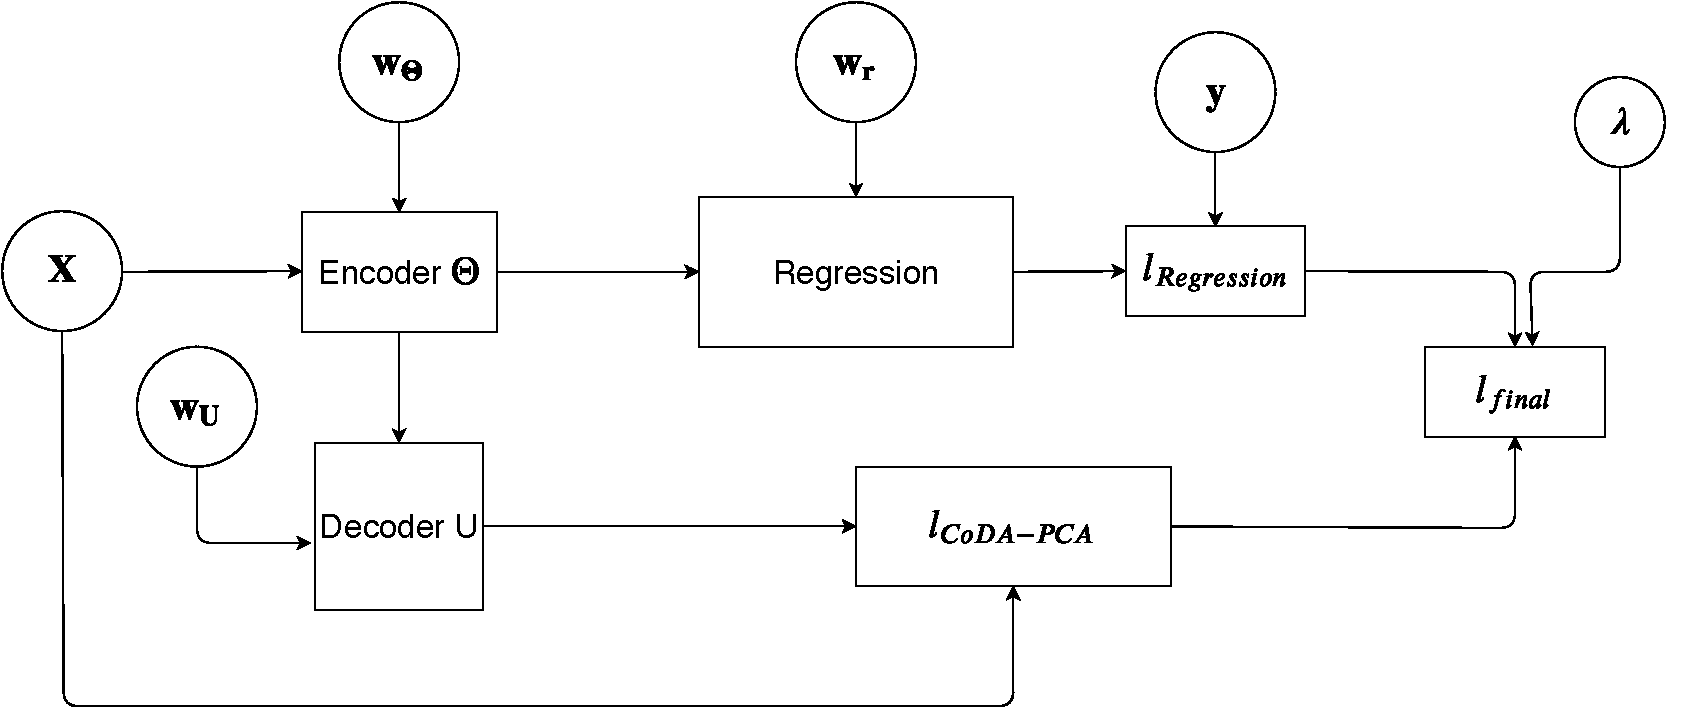
\includegraphics[width=17cm]{figs/codadiagram.pdf}
    \caption{End to End ("Coda-to-end") Model Diagram}
    \label{fig:model}
\end{figure}

% Description of symbols:\\
% $\bf X$: Input Matrix\\
% $\bf{w_\Theta}$: Parameters for Encoding Network \\
% $\bf{w_U}$: Parameters for Decoding Network\\
% $\bf{w_r}$: Parameters for Regression\\
% $\bf{y}$: Target vector\\
% $\lambda$: Regularisation parameter, controlling how much to weight reconstruction error
% \\\\





\section{Implementation}
\label{implementation}
The model defined in \ref{architecture} was implemented in PyTorch, with the source code available on GitHub. A high level outline of the implementation is as follows: The algorithms CoDA-Regress and CoDA-Cl form the basis for the code, and are each implemented as a separate class. The user defines the desired low level dimension, as well as the encoder and decoder dimensions. Using these parameters, an ordered dictionary is used to stack the layers for the encoder and decoder to ensure the correct ordering of dimensions. This includes the nonlinearities, for which we use Exponential Linear Units (ELUs). These dictionaries are then used as input to the  PyTorch Sequential module to format them as PyTorch objects. \\

The output layer is algorithm specific. CoDA-Regress has a linear layer mapping to a single output, which is the predicted regression value. CoDA-Cl has a linear layer mapping to the number of classes followed by a log softmax layer, which gives the log probabilities for each class. \\

The forward pass is as described in \ref{architecture}, with the input being modified to contain both the original matrix $X$ and $X_{ckl} = \log \check{X}$. This is done as per \cite{Avalos2018}. \\

The optimisation is done using Adam \citep{}. Referring to algorithm \ref{Alg1}, this takes the place of the function $O$. We found this to be more numerically stable during experiments in comparison to standard Stochastic Gradient Descent (SGD), in addition to faster convergence. 

\subsection{CoDA-PCA Package}

We see from \citep{Avalos2018}, CoDA-PCA gives a significant improvement in dimensionality reduction over current methods. Although the code for this paper is available, it has not yet been packaged to production standards. We have reimplemented and packaged the code from \citep{Avalos2018}, along with the CoDA-Regress and CoDA-CL algorithms presented here. These are available on the Python Packaging Index (PyPI), with easy installation using pip. These algorithms can be accessed using a simple API, which allows users to benefit from their advantages over related algorithms.   \todo{add documentation etc. of package?}



\section{Summary}
We have introduced the algorithms CoDA-Regress and CoDA-Cl for supervised learning problems with compositional features. 
Given a feature vector $\bf X$ and target vector $\bf y$, these models fit predictions using a low dimensional representation of the original data. The final loss is computed as the sum of the supervised loss $l_{y}$ and the reconstruction loss $l_{x}$, with the reconstruction loss being scaled by a real valued parameter $\lambda$.  




\chapter{Experimental Methodology}
\label{cha:methodology}

\subsection{Experiments}
In this section we present the results from experiments on the combined model. Experiments were done for both regression and classification tasks using several data sources. We present the results of our model in comparison to several baselines on each of these sources. 

\subsubsection{Model Evaluation}
The results for the smaller Aitchinson datasets were obtained using  k-fold cross validation combined with an inner hyperparameter selection loop. 

K-Fold cross validation is the standard approach for model evaluation in most machine learning contexts. The procedure is as follows: Choose $k$, which is the number of groups to split the data into. Shuffle the data, split into $k$ groups and take one as the test set. Train the model on the $k-1$ groups, and evaluate the performance on the test set. Repeat this procedure, changing which group is used for the test set. 

This approach is highly unbiased, since the data is shuffled and so trained and tested on separate partitions of the data. In order for the model to perform well overall, it must do well on each partition of the data. This prevents a good model score being due to a lucky initial testing split. Likewise, if a model performs well on only some splits, then this suggests it does not generalise well.  

Given the sensitivity of our model to the choice of $\lambda$, one solution is to use K-Fold cross validation with an additional inner loop for hyperparameter selection. The high level idea of this approach is as follows: Given a set of hyperparameters $\Lambda = \{\lambda_1 ,.., \lambda_n\}$. For each training partition of the initial K-Fold, $X_k$ we do another cross validation of $X_k$, for each $\lambda \in \Lambda$. The value of $\lambda$ which results in the best mean cross validation score is then used to train the model on $X_k$. Since we still do not have access to the testing data, this method will still give valid results. There is a large computational cost to this approach, with training taking $O(k|\Lambda|)$. This method, found in \cite{walder} is primarily useful for small datasets, due to the high associated computational costs. As such, it was performed on the initial testing of the model with the Aitchinson data.     

\begin{figure*}
    \centering
    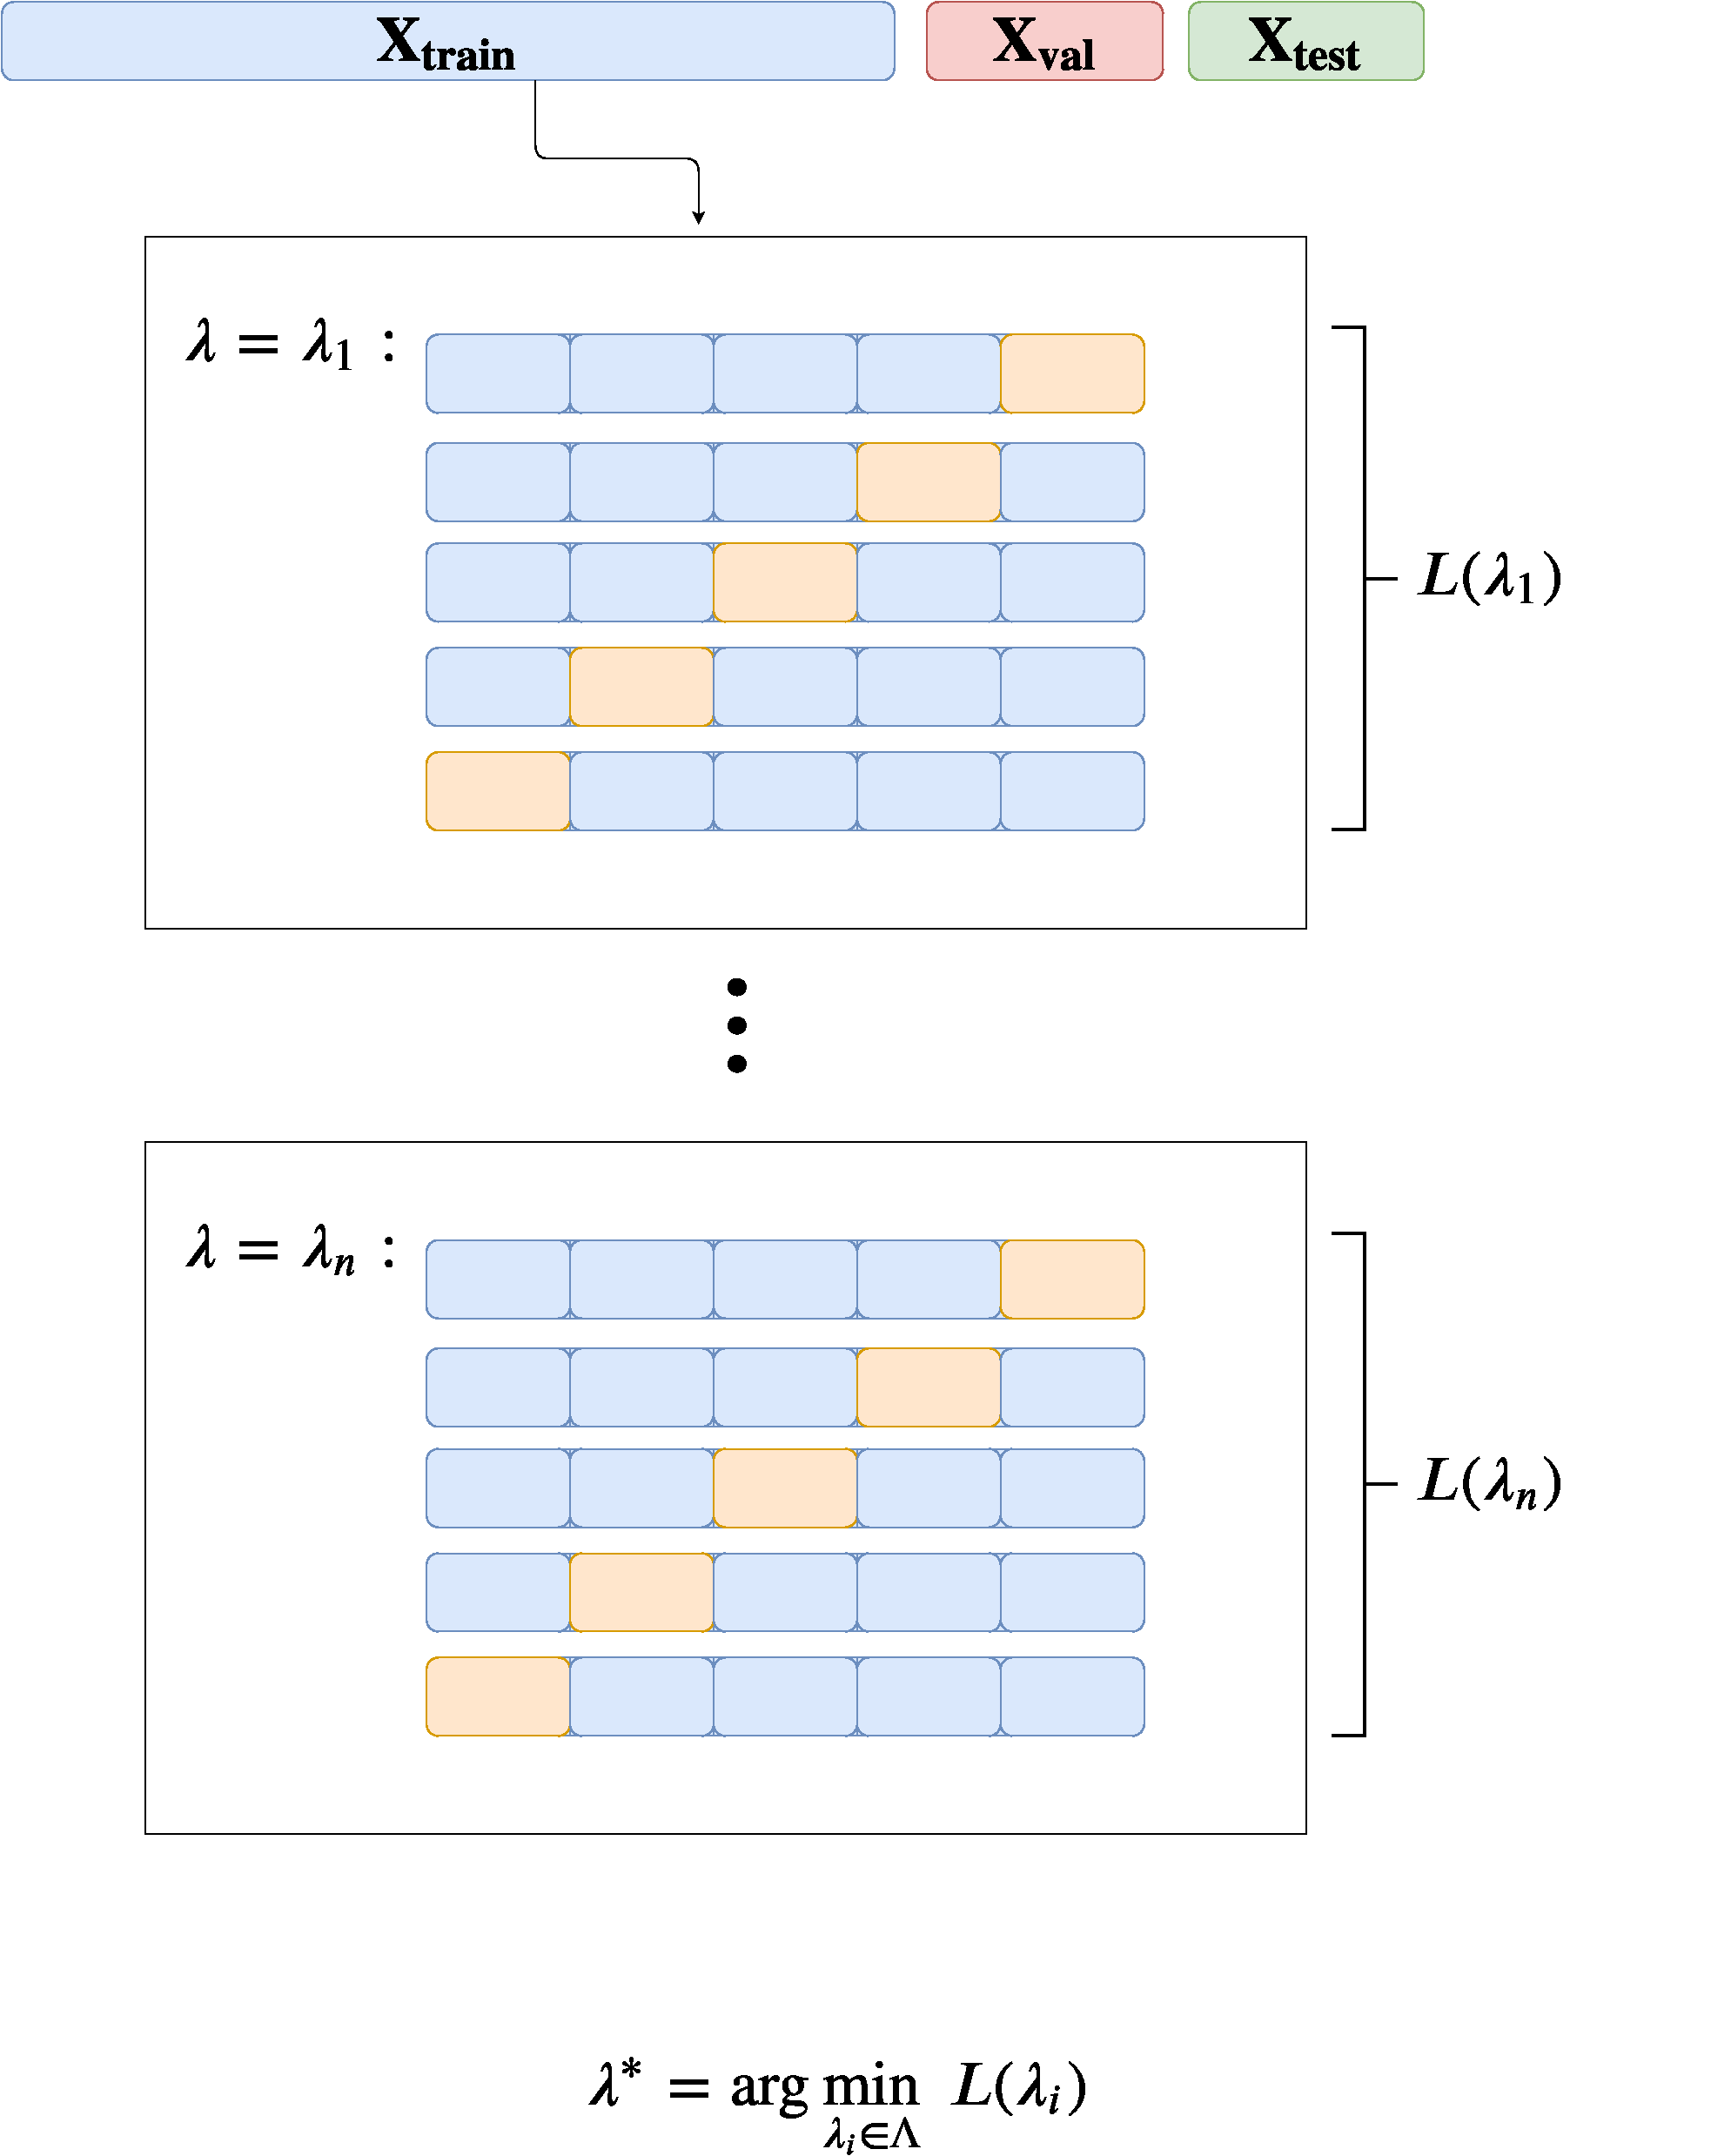
\includegraphics[width = \columnwidth]{figs/cross_val(1)(1).pdf}
    \caption{Hyperparameter selection loop for model evaluation: $\mathbf{X_{train}}$ is partitioned (here into 5). The final $\lambda^*$ is selected as the best performing $\lambda_i$ on the mean inner cross validation score, $L(\lambda_i)$. $\lambda^*$ is then used for training on $\mathbf{X_{train}}$, and this is repeated for each training split in the outer cross validation loop. }
    \label{fig:cross_val}
\end{figure*}

\subsection{Data Sources}

\subsubsection{Aitchinson Data}
The first data source that we test on is the supplementary data presented by Aitchinson [ref.]. This data is commonly used in CoDA research, and consists of 40 small sample (up to 92) compositional datasets. As part of this project, this data was digitised and uploaded to Zenodo. Zenodo is an open access research repository, and so this will allow other researchers to easily access this data in the future. The digitised data can be found here..  


\subsubsection{Metagenome Data}
The next source was from a recent paper in Nature \citep{Stewart2019}, which provided the metagenome analyses from several hundred cattle rumen. The depth of each genome (which acts as a proxy for species count) is given for each of the cattle in the sample. The collection of depths per cattle is compositional due to the capacity of the sequencing device being limited, as we saw from \cite{Gloor2017}. There were 4941 genomes identified between the 283 cattle. This data provides a good opportunity for testing the model on high dimensional data, since $d >> n$ for dimension $d$ and sample size $n$.  

\subsubsection{Additional Microbiome Data}


\subsection{Model Tuning}
\subsubsection{Early Stopping}
Add figures and cross val results showing dip in training loss, increase in val loss and decrease in cross val performance
A useful technique in the training of machine learning algorithms is early stopping. This is often employed to reduce model overfitting, as the model weights can become overly optimised on the training data if trained for too long, and so lose their ability to generalise. Early stopping is a simple solution to this; it terminates the training early if the training and validation loss diverge. 



\subsubsection{Numerical Stability}
The implementation of Machine Learning algorithms on digital computers often leads to numerical instability. Given that real numbers can only be approximated to a finite precision with floating point numbers, operations on very large or small numbers can lead to numbers beyond the scope of this representation. In addition, the finite precision means that there is an inherent error associated with operations on these numbers. These errors accumulate, and can lead to results which do not align with what it would be analytically. Even when a high precision is used, it is well known that matrix operations are particularly prone to numerical instability. Given that these form the basis for many machine learning algorithms, numerical analysis is an important consideration.

clamping, NaN, exploding gradients, vanishing gradients, learning rates, local optima 














%%% Local Variables: 
%%% mode: latex
%%% TeX-master: "paper"
%%% End: 

\chapter{Results}
\label{cha:result}
Experiments \fix{TODO}
In this chapter we present the results of the experiments performed on the end to end model in \ref{design}. The goal of this section is to  present the conditions under which this type of model performs well, and likewise to determine when it does not. 

\begin{itemize}
    \item Section \ref{toygauss}: This section covers the application of our model to a simple toy dataset, designed to test the hypothesised advantages over traditional methods.
    
 
\end{itemize} \pagebreak



\section{Toy Example: Gaussian data}
\label{toygauss}
%https://link.springer.com/content/pdf/10.1023%2FA%3A1023818214614.pdf 
for creating compositional data with orthonormal bases

The first situation where we will test our model is a synthetic dataset. We want this data constructed in such a way as to test the underlying hypothesis motivating the model in \ref{design}. That is, our end to end model can improve performance in cases where standard dimensionality reduction removes potentially useful information.

In order to appropriately test this, we therefore want our data to contain useful information which we expect standard methods to ignore. The approach we take to construct this is to take a $d$ dimensional Gaussian, with mutually independent components for simplicity. The covariance matrix is then composed of the diagonal variance entries of each dimension. The important point here is to set the variance of each dimension to be largely different in magnitude. Since the covariance between dimensions is zero, we would expect the coordinate system of dimensionality reduction methods to be focused on the axes with the largest variance. We expect this coordinate system to contain little information on the lower variance dimensions.  If the supervised learning target is a function of these lower dimensions, we would therefore expect to see low performance when using these as features. In contrast, the use of a combined model has the signal of supervised loss as a factor in the choice of representation. It should choose a representation which still preserves the important information in the lower variance features. So we expect to see an improvement in performance for this type of data when using our model in comparison to baseline methods. \\

Formally, we generate this data by taking $n$ draws from a $d$ dimensional Gaussian denoting the variance for each component (i.e. the diagonals of the covariance matrix) as $\sigma_1, ..., \sigma_d$. From above, we note that $\sigma_1 >>  ... >> \sigma_d$. Then we define our $n\times d$ data matrix $\mathbf{X}$, with each $\mathbf{x}_i \sim \mathcal{N}(\mathbf{0}, \Sigma)$. Since CoDA requires non-negative values, we scale each axis by the minimum value if it is negative. Our targets will then be a function of the least variant axis, $\mathbf{y} = f(\mathbf{x}_j), j = 1,...,d$ (where $j$ is indexing $\mathbf{X}$ by columns i.e. axes).  \\

Figure \ref{} shows an example of synthetic data constructed in such a way. We note the large difference in the spread of the data between the axes, and 


Implementing this, we 

From our results, we can clearly see the advantage of an end to end model over baselines when the targets are a function of the least variant axis. An interesting experiment to follow this is to invetigate how this performance differential changes as the targets become a function of more variant axes. 

add results 

discuss

\subsection{Hyperparameter Grid Search}
Below we present the results from the 3 trial hyperparameter grid search protocol we introduced in \ref{cha:methodology}.  





\section{CoDA-PCA Microbiome data}
Smallish for both dimensions, uses OTUs at genus level

Still no improvement over baseline using end to end. Even with larger sample size (1000), performance is at best the same, often much lower.  

\section{RUG}
New microbiome results, using species level  
- Poor performance, can't do better than chance
- Why?: Sheer depth of connections needed in 'fat' matrices to map them to a lower dimension. The small sample size does not allow for enough information for the network to establish meaningful relationships between the input, low level representation and the output. 
- Preprocessing with dim reduction works better because the dimensionality reduction algorithms are fixed, and there is no need to learn them unlike in the network.
- Can see from 2D/3D plots there is not enough information in these dimensions to meaningfully distinguish classes. Also note the different representations of PCA and CoDA-PCA

A lot of modern results are of this 'fat' form, given the small sample sizes and large diversity in microbiome species. To improve performance/reduce size it may make sense to do analysis at the genus or higher level. 

https://microbiomedb.org/mbio/app/ other sources if needed

%\section{Direct Cost}\
%\label{sec:direct_cost}

%Here is the example to show how to include a figure. %Figure~\ref{fig:cost}
%includes two subfigures (Figure~\ref{fig:zerocost}, and %Figure~\ref{fig:zerobus});

%\begin{figure*}
%  \label{fig:cost}
%  \subfigure[Fraction of cycles spent on %zeroing\label{fig:zerocost}]{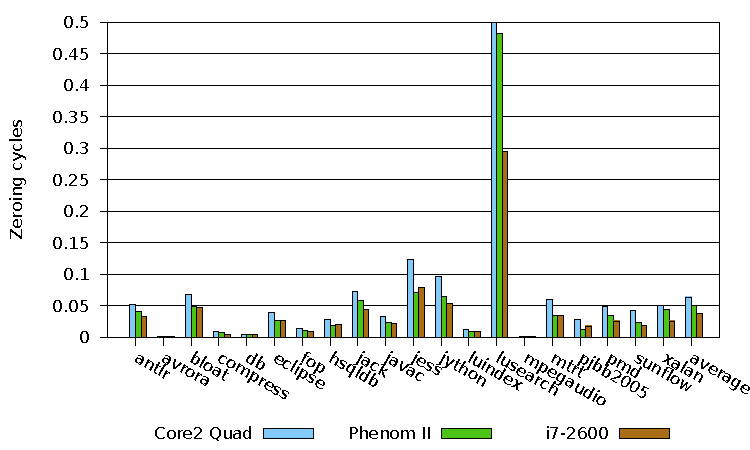
\includegraphics[width=\columnwidth]{f%igs/zerocost_intel.pdf}}
%  \subfigure[BytesZeroed / %BytesBurstTransactionsTransferred\label{fig:zerobus}]{\includegraph%ics[width=1.0\columnwidth]{figs/zerobus_core.pdf}}
%  \caption{The cost of zero initialization}
%\end{figure*}


\section{Summary}

\chapter{Conclusion}
\label{cha:conc}
Summary your thesis and discuss what you are going to do in the future in Section~\ref{sec:future}.


\section{Future Work}
\label{sec:future}
Good luck.





%%%%%%%%%%%%%%%%%%%%%%%%%%%%%%%%%%%%%%%%%%%%%%%%%%%%%%%%%%%%%%%%%%%%%%
% Here begins the end matter

%%% \appendix

\backmatter

\bibliographystyle{anuthesis}
\bibliography{thesis}

\printindex

\end{document}
